% A simple template for LaTeX documents
% 
% To produce pdf run:
%   $ pdflatex paper.tex 
%


\documentclass[12pt]{article}

% Begin paragraphs with new line
\usepackage{parskip}  

% Change margin size
\usepackage[margin=1in]{geometry}   

% Graphics Example:  (PDF's make for good plots)
\usepackage{graphicx}               
% \centerline{\includegraphics{figure.pdf}}

% subfigures, side by side
\usepackage{subcaption}

% hyperlinks
\usepackage{hyperref}

% Blocks of code
\usepackage{listings}
\lstset{basicstyle=\ttfamily, title=\lstname}
% Insert code like this. replace `plot.R` with file name.
% \lstinputlisting{plot.R}

% Monospaced fonts
%\usepackage{inconsolata}
% GNU \texttt{make} is a nice tool.

% Supports proof environment
\usepackage{amsthm}

% Allows writing \implies and align*
\usepackage{amsmath}

% Allows mathbb{R}
\usepackage{amsfonts}

% Numbers in scientific notation
% \usepackage{siunitx}

% Use tables generated by pandas
\usepackage{booktabs}

% Allows umlaut and non ascii characters
\usepackage[utf8]{inputenc}

% norm and infinity norm
\newcommand{\norm}[1]{\left\lVert#1\right\rVert}
\newcommand{\inorm}[1]{\left\lVert#1\right\rVert_\infty}

% Statistics essentials
\newcommand{\iid}{\text{ iid }}
\newcommand{\Exp}{\operatorname{E}}
\newcommand{\Var}{\operatorname{Var}}
\newcommand{\Cov}{\operatorname{Cov}}


%%%%%%%%%%%%%%%%%%%%%%%%%%%%%%%%%%%%%%%%%%%%%%%%%%%%%%%%%%%%

\begin{document}

\title{Code Analysis Project Proposal}
\date{\today}
\author{Clark Fitzgerald}
\maketitle

\begin{abstract}

\end{abstract}

\section{Introduction}
%%%%%%%%%%%%%%%%%%%%%%%%%%%%%%%%%%%%%%%%%%%%%%%%%%%%%%%%%%%%

The idea behind code analysis is to treat the code itself as a data
structure. This is an old idea, the R language reference cites the Lisp
language as the inspiration.

The interpreter works in a simple way. The \texttt{Rscript} command will go
through a file line by line and parses then
evaluates each statement. R's \texttt{source()} function on the other hand
first parses the whole thing, and then evaluates it all. We propose to
first parse and then examine whole scripts at a time, from just a couple
lines to a few hundred lines of code.  The whole script is parsed into a
directed graph data structure. Nodes contain the expressions and the edges
contain the dependence information.  TODO: but what about control flow?
loops?

Big point- Compilers have used all manners of static analysis and
intermediate optimizations to create more efficient code. Interpreted
languages are much more limited. But why not build refactoring tools that
can improve the performance?

Why this matters. It's reasonable to try to improve code performance if
slow speed affects many users. For scripts, superficially it might appear
that few people are affected. Indeed, if a researcher writes one script that
takes a couple minutes to run, and they run it a couple times then it
doesn't matter much, and there's no point in attempting to accelerate it.
However, these same sorts of "scripts" can be used in more serious ways.
For example, scripts can be used as Extract Transform Load (ETL) tools that
run as batch jobs every day or every hour. Then the script runs
many times, so it's important to realize more performance. For
ease of use and maintainability it's nice to have automatic tools to
accelerate the performance. One can write natural, beginner level scripts
and have them run much faster.

On a broader note, this is about embedding more intelligence into the code
and the system. As an end user it's convenient if a system will just ``do
the right thing'', or adjust to different work loads and data sizes on the
fly. I rarely know if something will be more efficient if
run with a multicore lapply versus a regular lapply. Then it would be
better for me if the system chose the right one for me.

How well will all of this handle non standard evaluation and different
paradigms like dplyr and pipes?

\section{Dependencies}
%%%%%%%%%%%%%%%%%%%%%%%%%%%%%%%%%%%%%%%%%%%%%%%%%%%%%%%%%%%%

We need to start out with some definitions and basic concepts to make all
of this precise. The following material is from the R
Language Reference \cite{Rlang}.

``A \textbf{statement} is a
syntactically correct collection of tokens.'' Less formally one can think of
a statement as a single line of code. The `line' rule doesn't always hold in practice,
since a semicolon can put two statements on one line, and a single
statement may span multiple lines.

\begin{verbatim}
# Two statements on line
a <- 1; b <- 2

# One statement on multiple lines
plot(lm(y ~ x,
        data = xydata))
\end{verbatim}

\textbf{symbol} is a variable name such as \textbf{a, b} above.  The words
symbol, variable, and name are used interchangeably. For consistency I'll
stick with symbol.

Assignment is the binding of a symbol to an R object. Complex assignment

``An \textbf{expression} contains one or more statements.'' Expression objects
in the langauge contain parsed but unevaluated statements. 

Statements can be grouped together using braces to form a \textbf{block}.
Since expressions can be nested, we can consider a block just a special
type of expression.

\begin{verbatim}
{
a <- 1
b <- 2
}
\end{verbatim}

TODO: Not sure how to handle blocks. One option is to go inside them and
look at all the individual statements. The other option, which seems easier
at first, is to do what CodeDepends does and group them into one
single logical unit. Presumably if a programmer writes a block like this
they intend the whole thing to execute together. One typically sees blocks
along with \texttt{if} statements.

But in the end I think I'll have to recurse inside the expressions at the
script level, but not down into the supporting library R code. For example, to
get a minimum set of code to perform a final operation one would need to go
into a block.

So how do we detect dependencies in code?

Idea talking with math students- count the incoming and outgoing edges. Use
this info.

\section{Graph Construction}

The graphs can be built sequentially, as the script is parsed.

The nodes in the graph are code expressions.
An expression may do any combination of the following things:
\begin{enumerate}
    \item Define new symbols
    \item Use existing symbols
    \item Redefine existing symbols
\end{enumerate}

Consider the following simple script:

\begin{verbatim}
x <- 1:10   # expression 1
plot(x)     # expression 2
x <- 1:5    # expression 3
plot(x)     # expression 4
\end{verbatim}

The first expression defines the new symbol \texttt{x}. The third
expression redefines \texttt{x} without making use of the existing
definition.

The second expression uses \texttt{x}, so we define an edge from node 1 to 2.
More generally we define an edge from the most recent expression that
updated \texttt{x}. Therefore the fourth expression creates an edge from 3
to 4.

The complete graph is then:

\begin{verbatim}
1 -> 2
3 -> 4
\end{verbatim}

But how will we know if the symbol exists? After parsing we could
potentially see the timelines recording which symbols live, and if they are
ever removed. This may depend on conditional statements, which we can't
know. The safe thing then seems to just assume that they will be used.

TODO: Is this just for the global namespace? How will it be different for
others? I think it's ok to just focus on the globals first. Environments in
general may require more thought.

``R adheres to a set of rules that are called lexical scope. This means the
variable bindings in effect at the time the expression was created are used
to provide values for any unbound symbols in the expression.''
\cite{Rlang} A primary goal is to respect R's lexical scoping rules.

Let $k$ be the number of cores on a machine.
To accelerate code by running in parallel the best possible case is if
we can keep all $k$ cores busy at once. This will happen if there are $nk$
expressions which can be independently scheduled for some positive integer
$n$. Additionaly, each expression should take long enough that
it's worth the overhead of using an additional R process to evaluate it.
On a two core machine that script might look something like:

\begin{verbatim}
# These could be run in parallel
a <- long_running_func()
b <- long_running_func()
\end{verbatim}

Side note- where exactly is the overhead of using multiple processes? Is
there latency? There's certainly a limit to how much data we move.

The worst possible case is if the second long running computation depends
on the first, and everything else depends on the second. Then it must run
in serial so multiprocessing can't help.

\begin{verbatim}
a <- long_running_func()
b <- long_running_func2(a)  # depends on a
# Now perform many operations on b
\end{verbatim}

\section{Optimization Problem}
%%%%%%%%%%%%%%%%%%%%%%%%%%%%%%%%%%%%%%%%%%%%%%%%%%%%%%%%%%%%

Consider the problem of whether or not to run blocks of code in parallel.
I'm thinking of this as an integer programming problem. 
The directed edges in the graph are the constraints, ie. an edge $A
\rightarrow B$ implies that $A$ must happen before $B$.

It resembles a
variation of a scheduling problem. The main constraints are that any variables
used in one computation must be available when it begins to run. Another
constraint is that k cores can be active at one time.

The other way general way to do this is running with several different data sizes. This
gives us a sample that we can run statistics on.

\section{Code graph and parse tree }
%%%%%%%%%%%%%%%%%%%%%%%%%%%%%%%%%%%%%%%%%%%%%%%%%%%%%%%%%%%%

I want a data structure that captures all of the constraints for the order
in which the code statements must be run. Preferably the minimal
set of constraints.

The constraints are implicit based on the order of the statements in the
code. This is a way of expanding and looking more carefully at this
implicit logic.

The code graph and related data structures are related to the parsed
script, which we'll refer to as the \textbf{parse tree}. Since the parser
doesn't care about spaces, tabs, and comments,  different scripts can produce the same parse
tree. R's \texttt{getParseData()} preserves all of the source
information, and this can be very helpful for debugging or IDE's. Later
this might be useful for injecting code.
For our immediate purposes scripts differing only in comments and white space can be
considered the same, which gives a 1 to 1 relationship between scripts and
parse trees. 

Many parse trees can give rise to the same code graph. For
example, the code graph shouldn't care if one uses \texttt{<-} or
\texttt{=} for assignment. Nor will it care about the ordering of two
adjacent lines binding a symbol to a literal constant:

\begin{verbatim}
a <- 1
b <- 2
\end{verbatim}

Therefore we lose information by converting from a parse tree to this code
graph.

\lstinputlisting[language=R, caption=Simple script, label=list:ab]{../experiments/ast/ab.R}

\begin{figure}
\centering
\begin{subfigure}{.6\textwidth}
    \centering
    \includegraphics[width=.8\linewidth]{../experiments/ast/ast.pdf}
    \caption{Parse tree}
    \label{fig:ast}
\end{subfigure}%
\begin{subfigure}{.4\textwidth}
  \centering
  \includegraphics[width=.8\linewidth]{../experiments/ast/codegraph.pdf}
  \caption{Expression dependency graph}
  \label{fig:codegraph}
\end{subfigure}
\caption{Different representations of the script in Listing \ref{list:ab}}
%\label{fig:test}
\end{figure}

For visualizing the control flow and dependencies it's important to have the entire
expression available in the node as in Figure \ref{fig:codegraph}. This
lets users easily connect the graph with the source file. Another thought
that would make this easier- put the source code line number along with the
line of code.

Duncan was pointing out how I don't need the edge connecting the first line
to the last line in Figure \ref{fig:codegraph}, because it's implied by the
path through the intermediate node. True. So I could go through and remove
those edges. How to do that? Can a dominator tree help with this? It's nto
a

This would then help me see where the parallelism is, and put it in an
appropriate data structure. Once I do that I can collapse simple threads
consisting of chains of nodes with single inputs and outputs
down into something like this:

Looking at some of Nicks stuff- what I'm really thinking about is breaking
up the basic blocks into expressions and looking at relationships between
them, with parallelism as one potential end goal. He's looking
more carefully at the control flow implied by how the user wrote the code.

\begin{verbatim}
A may have many incoming edges, C may have many outgoing edges.

Then:
A -> B -> C   becomes a single node ABC
\end{verbatim}

This will preserve the semantics and the ideal parallelism. Proof?
It also leaves a data structure that's as simple as it can be, which is
what I'd want to use when actually modifying the source code.

But the task graph is not the same as control flow. Control flow is things
like for, while, return, etc. The task graph is a higher level construct. 
Nodes are R expressions that appear at the top level of a script, which
means all control flow is captured \emph{inside} a node. Create an edge
from node $A$ to $B$ if $B$ uses a variable that was most recently updated
in $A$. There is some ambiguiity here, since variables may be created
within conditional statements. In that case we can take the conservative
approach of just creating all the edges. An example:

\begin{verbatim}
# coinflip(p) randomly returns TRUE or FALSE with probability p
x <- 10
if(coinflip(p1)) x <- 20
if(coinflip(p2)) x <- 30
y <- x + 1
\end{verbatim}

Thinking harder about this, it is necessary that the assignments into the
global workspace happen in order. But it's not necessary that the code runs
in order, because the \texttt{if(coinflip())} lines don't use \texttt{x} as
an input. Then there are two types of constraints to have the correct
semantics- a weaker one for evaluation and a stronger one for assignment. 

Here's a related case:

\begin{verbatim}
x <- f(...)
x <- 10
y <- x + 1
\end{verbatim}

Here the line \texttt{x <- f(...)} is unneeded, as are all lines just done
in support of this operation. This suggests that as a first pass we would
want to identify and remove unnecessary code. Then we can assume every
line of code that remains needs to run. I'm also assuming that the code is
correct. Compared to other ways of accelerating code this requires
basically nothing from the user. So it's comparable to byte code
compilation in that
sense- just a small acceleration from minimal investment.

But is the task graph a DAG? Yes, I think it has to be, unless you're doing
something totally weird.  The reason is that R scripts execute
sequentially, they don't have a GOTO statement. It's true that loops can
repeat the same lines of code many times, but \texttt{for()\{...\}} and 
\texttt{while()\{...\}} are just single top level expressions- we're not
expanding them out in the graph $n$ times. This is an argument in favor of
not recursing into these expressions- if we do then it opens up many
problems. 

One could make the argument that calling \texttt{source()} on some script
a couple different times in a program can make for repeated code which
causes trouble with the DAG. One way of handling this is to go read the
contents of the file being sourced, then consider this statement just like
any other- taking in variables and producing them.

We can also introduce an artificial (graph style) source and sink representing the
beginning and end of the program, respectively.

Variable updates don't need to be DAGS- but then again it doesn't make
perfect sense to talk about control flow in terms of variables.

\section{Task Graph Literature Review}
%%%%%%%%%%%%%%%%%%%%%%%%%%%%%%%%%%%%%%%%%%%%%%%%%%%%%%%%%%%%

Most of these highly cited papers seem to focus on making systems faster
and more efficient. What about the value of looking at a task graph for
educational / explanation purposes?

Ferrante et. al. introduce the program dependence graph.
\cite{ferrante1987}. The approach I'm looking at now should be higher level
than this, because this explicitly handles control flow. I can get out of
this by only looking at the top level statements in a script. The control
flow there is super simple- all the statements execute in order!

TODO: see which graph definitions we can borrow from this and other papers-
ie. ``hammock''.

\cite{cosnard1995automatic} describe constructing a task graph based on
annotating the source code the program. They go into every iteration of the
loop, which differes from what I'm proposing.

\cite{adve2004parallel} presents a model for predicting the run time of
programs based on a task graph. 
Their definitions on page 98 are nice and clear, I should use them.
Based on the graphs of their figures the
programs seem very like very regular, well defined algorithmic programs. A
general data analysis script in R is probably much more variable than this.

This is one way to distinguish and justify my work here as different from
CS- general forms of scripting and data analysis are usually quite
different than a pure focus on algorithms.

Nice explanation of program dependence graph (PDG):

\begin{quote}
    A PDG node represents
    an arbitrary sequential computation (e.g., a basic block, a
    statement, or an operation). An edge in a PDG represents
    a control dependence or a data dependence. PDGs do not
    contain any artificial sequencing constraints from the
    program text; they reveal the ideal parallelism in a
    program. \cite{sarkar1991automatic} 
\end{quote}

We can borrow their idea of distinguishing ideal parallelism from useful
parallelism. Overhead makes these two different.

The hierarchical task graph was introduced in \cite{girkar1992automatic}
for the purpose of detecting task parallelism in source code for use in compilers.
As in the others, it incorporates the control flow for a fine grained
parallelism. They allow `compound nodes' containing nested htg's.

As of 2009, most efforts to parallelize R have focused on the lower level
programming mechanisms. These needed to be in place before any higher level
automatic detection could be built and function.
\cite{schmidberger2009state} 

What I'm looking at is very close to the Use-define chain.
\url{https://en.wikipedia.org/wiki/Use-define_chain}. But I'm staying just
slightly higher level. The hope is that staying at a high level will make
this more productive / easier to reason about and use than a low level
thing that examines every bit of control flow.

The Use-definition chain has been around since at least 1978
when it was used to remove dead (unused) code\cite{kennedy1978use}. This
reference has a nice consideration of what makes a computation useful or
not. It defines it recursively- something is useful if it's used later by another
computation. This is combined with the ``base case'' of usefulness- there's
a set of operations that are considered intrinsically useful. This author
considers calls to subroutines and branch test instructions as
intrinsically useful. We might take this idea and tweak it a little- define
R expressions as intrinsically useful if they have a side effect, ie. any
plotting commands, saving data to disk, etc.

So I wonder how much this has to be tied to R? CodeDepends is of course
purely for R. But other tools exist to manipulate parse trees independently
of any language, for example
\url{https://github.com/tree-sitter/tree-sitter}. Differences among
languages... it would have to recognize that a Python methods often mutate
their objects, for example:

\begin{verbatim}
x = [3, 1, 2]
x.sort()        # Sorts x in place, returning None
\end{verbatim}

LLVM has some functionality for working with these use / def chains
\cite{Lattner2004}. For example:
\url{http://llvm.org/docs/ProgrammersManual.html#iterating-over-def-use-use-def-chains}.
Following their terminology, an object of class \texttt{Value} is used by
potentially many objects of class \texttt{User}. The \emph{def-use} chain
is the list of all \texttt{Users} for a particular \texttt{Value}. I think
of this as all the places in the code where this variable propagates. In
contrast, the \emph{use-def} chain is the list of all \texttt{Values} for a
particular \texttt{User}. This is all the inputs to a newly
created object. There's room for both of these chains to be expanded recursively.

In this example the def-use chain for \texttt{x} is only \texttt{[y]}, but the
recursive one is \texttt{[y, z, z2]}. The use-def chain for \texttt{y} is
\texttt{[z, z2]}.

\begin{verbatim}
x = 10
y = x + 5
z = y + 2
z2 = y + 100
\end{verbatim}

We might be able to use this along with R code to determine if an R
function calling C code is pure.

\section{How CodeDepends works}
%%%%%%%%%%%%%%%%%%%%%%%%%%%%%%%%%%%%%%%%%%%%%%%%%%%%%%%%%%%%

The parsing uses an object oriented wrapper around R's builtin \texttt{parse()}
which handles different file types ie. script or dynamic documents among other arguments.
This doesn't directly expose code comments.
At first glance it seems CodeDepends uses the tokens
more indirectly, through functions like \texttt{is.name()}. 

The workhorse functions are in \texttt{CodeDepends.R}. Overall, the
approach resembles \texttt{codetools::walkCode} as discussed in
\ref{chambers2016extending}. Essentially it walks the tree of code, calling
a function to collect usage information.

When analyzing a single expression, first a 
collector object is created with \texttt{inputCollector()}. This is a
closure that maintains a list of everything in the expression that has been seen
so far: files, variables, function calls, etc. It returns a list of
functions to update the data in the closure.

\texttt{getInputs.language()} takes a collector object and
recurses through expressions until it finds the leaf nodes which can be functions, calls, assignments,
names, literals, or pairlists. Upon finding one of these leaf nodes it
calls the collector object. 
Many special cases of functions are handled in functionHandlers.R, such as
\texttt{\$, rm, for} as well as non standard evaluation. Special attention seems
to have been paid to dplyr operations.

As a user I'd like a clean, well defined entry point and API for this
stuff. The problem I had today was trying to pass arguments into
\texttt{inputCollector}. I did this by hacking through the code of
\texttt{makeTaskGraph}.

TODO: Ask Duncan where the separation between CodeDepends and CodeAnalysis
should be. How about makeTaskGraph? Probably first I should just look more
in CodeAnalysis to see what's there.

The \texttt{ScriptNodeInfo} objects contain all processed information about
each expression. They tell which variables 

\section{Related Work}
%%%%%%%%%%%%%%%%%%%%%%%%%%%%%%%%%%%%%%%%%%%%%%%%%%%%%%%%%%%%

Jim Hester's covr package \cite{R-covr} checks unit test coverage of R
code. It is a practical example of computing on the language,
programmatically modifying the code by recording calls as they are made.
He pointed out a nice relevant idea distinguishing between AST's, parse
trees, and "lossless syntax trees":
\url{https://news.ycombinator.com/item?id=13628412}. If I inject code then
I need to careful preserve structure lost after parsing, ie.
comments and formatting. This is a non-trivial task.

So if I'm going to programmatically modify the source code then this should really
respect things like comments and whitespace. This could be more difficult
than it appears on the surface.

TODO Gives me an idea... a similar strategy might work to collect timings and
resource usage for functions called with various data sizes. This could be
implemented with something like \texttt{System.time()}. We could
attach timings to each expression. Then we can
use this info to programmatically modify the code: ie. if $n > 1000$ then
run a multicore version. This is something like Profile Guided Optimization
(PGO). This technique is now being used for Python. Could R use it too?

Maybe a simpler way to do this is to just use the built in profiler. Use
the results to determine whether parallelization is worth it, and maybe set
some bounds for expected performance changes if one uses various forms of
parallelism. 

There may be potential to use statistical methods for this.
Run it many times, collecting profiling results for various values and use
this as the training data. After all, we have easy access to all the
machine learning type things that we need. We can use it to automatically
tune. But this implies that there is some way to tune it. Right now the
only "trick" I have up my sleeve is to try to parallelize it.

The vignette in Tierney's \texttt{proftools} package has some nice examples
of visualizing profiling data. The call graphs and related visualizations
are conceptually similar to what I have in mind.
Wickham's \texttt{profvis} integrates with the IDE to indicate the actual
line of source code along with the related timing info.

Knitr (TODO cite) facilitates reproducible computations for
chunks of code in Rmarkdown documents. One feature it enables is caching,
ie. it doesn't need to run a chunk of code if nothing has changed. One can
manually specify the chunk dependencies by relative or absolute indices,
ie. -2 for the chunk 2 blocks in front of the current chunk, or 1 for the
first chunk. This seems unreliable because it requires the user to
accurately infer the dependency information, and it doesn't automatically
adjust if one inserts new chunks in the document.

Knitr also has an \texttt{autodep} option to infer this dependency
information. This works by comparing the global variables existing before
and after running the code in each chunk. It stores this information in
special files. So it doesn't use any static analysis of the code.

But the structure of knitr blocks here is actually very appealing- this is
a great use case for the parallelism. Why not evaluate the chunks in
parallel if you can? I wonder how difficult it would be to hook into
knitr's system... And while I'm at it, why not Jupyter Notebooks? If I can
figure out how to build an equivalent dependency graph for Python that
would be great.

Henrik Bengston's \texttt{future} package provides a mechanism for
asynchronous evaluation of R expressions. Once I have a partial ordering
through the dependencies it
would be appealing to evaluate every code expression with this. 
futures mostly just provides the asynchronous
assignment operator \texttt{\%<-\%}. Then I'd have to go in every
expression and replace the regular assignment operators. This could lead to
lots of weird stuff- what if a for loop goes through and assigns 1000
times? That's a ton of overhead.

I'm thinking more seriously now about the networkspaces or linda spaces
evaluation model, like Mike Kane mentioned at DSC. This consists of a
single master server that sends code to a worker to evaluate to produce a
variable. It's like a key value store, except there can be multiple values.

So how would I make this happen?


\section{Applications}
%%%%%%%%%%%%%%%%%%%%%%%%%%%%%%%%%%%%%%%%%%%%%%%%%%%%%%%%%%%%

What are all the useful things to do when rewriting code?  Duncan's very
helpful docs here http://www.omegahat.net/CodeDepends/design.pdf give a
handful of reasons.

Other things that I can think of:

Identification and elimination of dead code.

- Given a big ugly script, pull out the minimal set of code to produce a
  final result. For example, everything needed to make `plot(finalresult)`.
- Parse Rhistory to find the minimal set of code to reproduce a result.
- Separate single scripts into multiple scripts if they actually have two
  independent sequences of computation.

These ideas stay much closer to the syntax and language of R compared to
what Nick is doing.

I've been considering this for the purpose of analyzing, accelerating and
optimizing essentially single scripts. But how important is this generally?
It only matters if someone's script runs slow. Probably this mostly happens
due to one large computation. If they're doing two large and independent
computations in one script shouldn't that be two scripts? But these tools
should be able to split them up at that level if I ask them to.

Remove all objects as soon as they're finished being used in the script. If
creating many large intermediate objects this could help with not using
excessive memory.

\section{Detecting Parallelism}
%%%%%%%%%%%%%%%%%%%%%%%%%%%%%%%%%%%%%%%%%%%%%%%%%%%%%%%%%%%%

Not sure how to generally detect where the possibilities for
parallel are. In a simple case of k obvious threads with one common
ancestor and common child there is an obvious option:

Remove the common ancestor and child and select the k disjoint subgraphs
between them.

Alternatively:

1. Start at the top of the graph, and move down until one node has
multiple children. Gather those child threads into 2 groups.
2. Same thing starting at the bottom.

The most straightforward thing to do right now is take a more complex
graph, say something like this:

\centerline{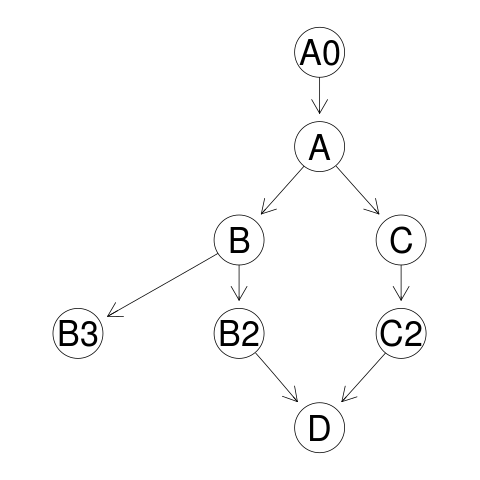
\includegraphics{../codedepends/larger_graph.png}}


And attempt to collapse the structure into one where the parallel threads
become obvious:

\centerline{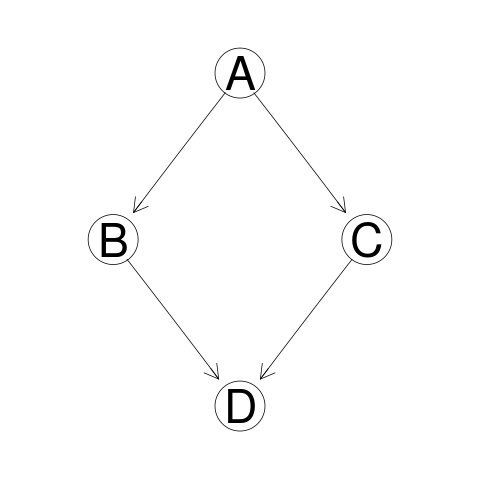
\includegraphics{../codedepends/simple_graph.png}}

The essential part for the multiprocessing is to have many "adjacent"
threads (is there a correct graph term for this?)
Optionally the adjacent threads can share a common parent and or child
nodes.

\section{The right data structure}
%%%%%%%%%%%%%%%%%%%%%%%%%%%%%%%%%%%%%%%%%%%%%%%%%%%%%%%%%%%%

I want to work with a DAG constraining the order in which the statements
must execute. This DAG can initially be built sequentially with the following
algorithm:

\begin{verbatim}
for statement in allstatements
    for input variable x in statement
        create an edge from the most recently seen statement which outputs x
\end{verbatim}

It's not sufficient to just draw a single edge for the most recently used
variable. This will make a tree, but then it won't necessarily contain all
the dependency info.

But why am I interested in this DAG? Maybe more interesting is the partial
ordering that comes from it. And the threads. So maybe I need to think
about how to go from the DAG to the partial ordering. Wikipedia article for
partially ordered sets cites the set of vertices of a DAG ordered by
reachability as an example.

TODO:
Can this be a tree? Yes. Is it always a tree? I don't think so... Maybe
once extraneous stuff is trimmed off?

If the intermediate variable `b` is not used anywhere we probably want to
collapse the following into a single block of code, since it has to happen
sequentially. Therefore adding `future` here can't help at all. Unless it
should happen at the same time as another block... then two blocks can
execute simulataneously.

\begin{verbatim}
# Begin block
a = 100
b = a + 5
c = sum(b)
# end block
\end{verbatim}

\section{Hard things}
%%%%%%%%%%%%%%%%%%%%%%%%%%%%%%%%%%%%%%%%%%%%%%%%%%%%%%%%%%%%

`fit = lm(y ~ x)` doesn't detect the dependency of `fit` on `x, y`.

Following the control flow for `lm` we see the following calls:
`model.matrix.lm`, `model.frame.default`, `as.formula`. But eventually this
`y ~ x` itself must be evaluated in which case `.Primitive("~")` is called,
which certainly does something weird. But what?

Haven't yet checked things like:
`<<-, assign`

Recursion? Iterating updates?

Random number generation across processes. I'll need to make sure that it's
possible to reproduce random things. In general it's not going to be the
same if it's single threaded or multithreaded, but this is true in general,
so I don't need to worry about it.

\begin{quote}
     The behaviour with ‘mc.set.seed = TRUE’ is different only if
     ‘RNGkind("L'Ecuyer-CMRG")’ has been selected.  Then each time a child
     is forked it is given the next stream (see ‘nextRNGStream’).  So if
     you select that generator, set a seed and call ‘mc.reset.stream’ just
     before the first use of ‘mcparallel’ the results of simulations will
     be reproducible provided the same tasks are given to the first,
     second, ...  forked process.

     -R documentation for parallel::mcparallel
\end{quote}

I'll need to think carefully about what happens with dynamic evaluation.
And a related idea, functions can use variables that don't yet exist- but this
is weird- I just need to preserve the correct order. Here's some examples:

\begin{verbatim}
f = function() 0        # 1
g = function() f() + 1  # 2
f = function() 10       # 3
g()                     # 4
\end{verbatim}

The last line returns 11, since it uses most recent version of f().
The current dependency graph imposes this partial order:

\begin{verbatim}
1 -> 2, 1 -> 3, 2 -> 4
\end{verbatim}

So the statements could be written in the following order while still respecting the
partial order:

\begin{verbatim}
f = function() 0        # 1
g = function() f() + 1  # 2
g()                     # 4
f = function() 10       # 3
\end{verbatim}

In this case the call to g() will incorrectly return 1 instead of 11.
Hence there is a ``hidden'' dependency implicit here: \texttt{3 -> 4}.

A couple ideas to get around this: inline functions defined in the script.
Think harder about when evaluation must happen.

\section{Language Requirements}
%%%%%%%%%%%%%%%%%%%%%%%%%%%%%%%%%%%%%%%%%%%%%%%%%%%%%%%%%%%%

What does a language need to provide to make this easy?

Looking only at languages that are not compiled.

Metaprogramming

Pass by value semantics

\section{Scripts in the Wild}
%%%%%%%%%%%%%%%%%%%%%%%%%%%%%%%%%%%%%%%%%%%%%%%%%%%%%%%%%%%%

I could do some analysis on scripts that I scrape to determine theoretical
bounds for the number of statements that must be run sequentially,
and the max number of concurrent workers. My example script I've been
working on has about 50 statements, and I think min number of sequential
statements is around 10. Need to check. This could motivate reducing
overhead though.

Duncan suggests to find R code that's unacceptably slow, and see what these
methods can do to improve it. So to get a better sense of theoretical
improvements I could execute the code in normal R and attach timings for
each expression. This would show me true lower bounds for the method. It
would also be quite interesting to have some sense of the distribution of
execution times for different types of code. I imagine it varies
dramatically, but there may be rough patterns. One result I'm expecting is
that just one or two lines dominate the total script run time. In which
case anything I do can't really help. Unless that line calls one function
and I can use this method on the one function.

Vignettes, including those found on bioconductor, are for instructional
purposes, so they're mostly simple and self contained. This isn't the use
case I'm targeting. They are nice because the data should be included with
the package, thus I have some hope of actually being able to run them if
needed.

To get some idea of the potential for speedup, if I have an unlimited
number of cores, no overhead, and each expression takes roughly the same
amount of time to execute then the script can run no faster than the length
of the longest path in the graph. Hence speedup will be the total number
of statements divided by the length of the longest path in the graph.
By the way, all of those assumptions are unreasonable.



\section{Implementation}
%%%%%%%%%%%%%%%%%%%%%%%%%%%%%%%%%%%%%%%%%%%%%%%%%%%%%%%%%%%%

At first I iterated over the blocks of code and gathered dependency info as
I went along. But then I switched the implementation to focus on the variables
themselves to make my code easier to reason about. It should be slightly
more efficient, but that's not really a concern yet.

I consider updates of a list to be changes to the global list variable.
Thus something like the following redefines x every time. 

\begin{verbatim}
    x = list()
    x$a = f(...)
    x$b = g(...)
\end{verbatim}
 
This is easy and safe to do, but it might be inefficient if \texttt{f, g}
are expensive functions, because they could be run in parallel. An
alternate way is to think of \texttt{x\$a} as a variable that depends on
the original \texttt{x}. But adding details like these isn't worth it to me
now, because it's not core to what I'm trying to accomplish.

Detail- Calls to \texttt{library} need to make it to the top of the graph. Maybe in
general I can adopt the \LaTeX idea of a preamble, or setup code. But what else would go
there besides library?

It would be nice if I could look at the R global environment, then
look at an updated environment after running a line of code and take this
as the update. 

\subsection{Event Loop}
%%%%%%%%%%%%%%%%%%%%%%%%%%%%%%%%%%%%%%%%%%%%%%%%%%%%%%%%%%%%

Thinking about how to run the whole thing in parallel now. I could use a
model where the master sends out expressions to workers to
evaluate. This would be through an event loop that pops expressions from a data
structure.

And forks every time. Then the master polls the workers to see
when they're finished. Though it would be better if the workers could send a
message saying when they're finished. Seems like I might be able to do this
with \texttt{parallel::sendMaster}.

The process forking every time will be quite inefficient. The more intelligent
thing to do is `pipeline' the operations, and send whole related blocks of
expressions to various processes to evaluate.

The processes spawned with \texttt{parallel::mcparallel} communicate
through an OS level pipe aka FIFO. This is why the function returns a vector of
length 2 called `fd` for file descriptor, among other things. These are the
file descriptors to the pipes

But this may open up a different opportunity for faster, lighter weight
threads? A main consideration with threads is that one doesn't want one
thread to mess up a the data structure while another is using using it. But
perhaps using this expression dependency information will let us make
guarantees about safety?

Or what about using something even lighter than threads- like coroutines or
callbacks? It might be possible to dig into the guts of R and make
something like this.

This approach is different than rewriting the script as I did before. It's appealing
because it can do dynamic load balancing.

But it's not clear which expressions to evaluate first. Maybe I should
first do the ones that have the most dependencies? If an expression has no
dependencies then one can do it at any time, even way later. But if there
are many dependencies then none of them can run until the parent is
evaluated. This will end up needing some data structure acting like a priority queue.

Here's an algorithm: Start by marking all direct descendants of the special
0 (start) node as ready. Let the workers begin evaluating these
expressions.

\begin{enumerate}
    \item Expression $e_i$ is evaluated and the results are available again
        on master.
    \item For each expression $e_j$ which depends directly on $e_i$: check
        if $e_j$ has no other existing parents then mark it as ready.
    \item Remove $e_i$ from the graph.
    \item Worker begins executing any of the nodes that are marked as ready.
\end{enumerate}

There's some nuance here by trying to keep each of $k$ workers as busy as
possible while still respecting the constraints. Ie. there may be
bottlenecks where only one worker can be active, but after that all the
others can go.

This algorithm could also be refined into a priority queue by keeping the ready
nodes in a heap, with the values determining the heap order as the number
of expressions that depend on that expression, directly or indirectly. This
is a little naive- it would be better to have timings of the code and do
something more optimal in terms of reducing run time.

\newpage
\newpage

\Section{Chunking}

The task based parallelism isn't as relevant to how people use R (and other
languages) for data processing. Instead
lets think more about chunking and data parallelism. 

Parallelism introduces additional overhead on top of what dynamic languages
already incur. A general strategy to minimize this overhead is to ``chunk''
the computations. For example, given 1000 parallel operations one might
partition these into chunks of size 100 so that they become 10 parallel
tasks \cite{matloff2015parallel}.

I can take the code in \cite{matloff2015parallel} and see how changing the
chunk sizes affects the run time. I could also do this with Python's dask.

It would be nice to run just a couple in serial on the master process and
make principled decisions about how to run based on these results. For
example:
\begin{itemize}
    \item Is it worth it to run in parallel?
    \item Should we chunk? What should the chunk sizes be?
    \item Reverse the order for better load balancing?
    \item Dynamic or static scheduling?
\end{itemize}

Usually none of these are known ahead of time.  They also depend on the
particular problem.  The only way to know if a chunking scheme will work is
to experiment with a similar problem, then check expectations for the next
one. I also expect that they vary across different machines.

The book mentions using large chunks in the beginning followed by small
chunks for superior load balancing.

\bibliographystyle{plain}
\bibliography{citations} 

\end{document}
